
\section{Proposed Solution}

\subsection{Problem Statement}
Industry 4.0 has brought together traditional operational technology and IT systems, resulting in new attack vectors \cite{dietzUnleashingDigitalTwin2020}. Furthermore, the literature review has also revealed two major challenges in Industry 4.0: speed and security. For example, in the power automation system, the minimum acceptable time between fault detection and control is sent to the power station must be as low as 4ms \cite{rajkumar_cyber_2020} in order to ensure a timely response. Besides, Digital Twin is a trending topic that started being used in Industry 4.0 for various applications including monitoring, testing, and simulation of operations. However, our literature review reveals that most researchers either recommend a traditional encryption algorithm to secure the communication channel between IoT devices. On the other hand, from a security perspective, computational and power limitations make it difficult for (I)IoT sensors to use traditional encryption algorithms. Due to these two reasons, it is essential to explore and implement  lightweight encryption schemes that meet the security requirements while maintaining the necessary speed and efficiency of these systems.

\subsection{Proposed Solution}
The (Industrial) Internet of Things ((I)IoT) devices are low-power and resource-constrained, which makes them incapable of running traditional cryptographic schemes such as AES. Regardless, these devices are widely used across a range of Industry 4.0 sectors, such as manufacturing, transportation, health, and power grids, for various applications. In addition, IoT sensors are an integral part of Digital Twin technology, in which they are used to collect and send data over wired or wireless channels.

In this paper, we propose efficient and lightweight cryptographic encryption and authentication schemes to enhance the security of the communication channel between the Digital Twin and its physical components over the MQTT protocol using a technique called payload encryption.

\textbf{\textit{Why Lightweight encryption}}:
Lightweight cryptography algorithms are designed to be efficient and fast, making them suitable for use in resource-constrained environments such as (I)IoT devices and embedded systems.
These algorithms can be used to secure data at transit and rest in (I)IoT devices, ensuring the confidentiality, integrity, and authenticity of data. Furthermore, they are essential in applications where \textbf{real-time} data processing and \textbf{low latency} are critical requirements.

The following diagrams \ref{fig:ps-archi} show the scheme of our proposed solution. 

\begin{figure}[H]
    \caption{Scheme of Proposed Solution}
    \centering
    \includesvg[width=\textwidth, height=40cm]{images/svg/ps-scheme-final.svg}
    % 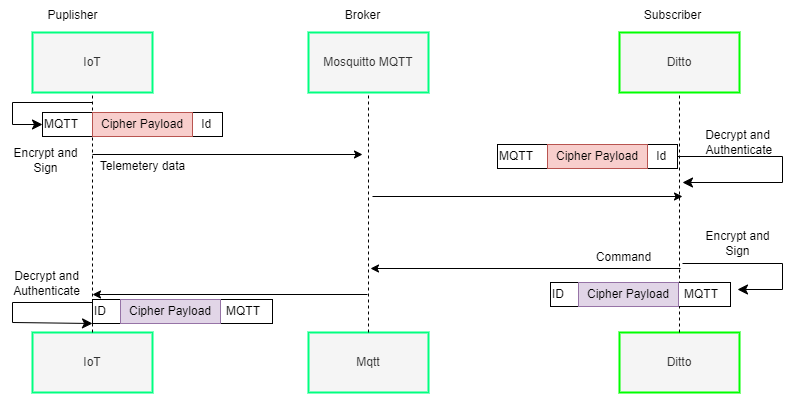
\includegraphics[width=\textwidth]{images/fp/payloadenc.drawio.png}
    \label{fig:ps-archi}
\end{figure}


\subsection{Research Questions}
In this second part of the master thesis, we aim to answer the following questions 
\begin{itemize}
    \item \textbf{RQ3} How to ensure the security requirement of digital communication between a Digital Twin and companion physical (I)IoT device?
    \item \textbf{RQ4} What is the performance analysis comparison of using the proposed lightweight encryption scheme and the existing solution presented(discussed) in the literature?
\end{itemize}


\subsection{Goal and Objectives}
The goal of this research is to implement and measure the performance of lightweight authentication and encryption schemes to address the security challenges faced by (I)IoT devices. The objectives of this study are to:

\begin{itemize}
    % \item Investigate the existing lightweight encryption schemes suitable for IIoT systems and assess their feasibility

    \item Select a NIST-standardised lightweight authentication/encryption scheme that can meet the security requirements of (I)IoT devices maintaining speed and efficiency.

    \item Implement mutual authentication/encryption scheme to secure a communication channel between a Digital Twin platform and a real (I)IoT device. 
    
    \item Implement an authentication/encryption scheme based on one of the traditional cryptographic algorithms. 

    \item Compare the performance of the proposed lightweight encryption scheme with one of the traditional encryption schemes.

\end{itemize}
This research aims to provide insight into resource-efficient security schemes for authentication and securing the communication between  (I)IoT  and DT applications in Industry 4.0 by achieving these objectives.




\subsection{Implementation Methodology}
To address research questions three (RQ3) and four (RQ4), we will select and implement an authentication/encryption scheme on
an open-source Digital Twin platform called Ditto and on one of micro-controllers called ESP32. The authentication/encryption scheme is based on a lightweight cryptographic algorithm standardized by NIST. 

Ditto is an open-source framework developed and maintained by Eclipse Foundation to facilitate the interaction between Digital Twin and IoT devices\cite{noauthor_eclipse_nodate}. On the other hand, ESP32 is a micro-controller chip manufactured by the Espressif system. 

To answer the last research question(RQ4), we will test our implementation
using a power measuring tool to estimate the performance of the proposed schemes in terms of power
consumption, execution time, and storage complexity. 

% \subsection{Plan}
% The anticipated timeline for this project is between 4 to 6 months. The first part of the project focuses on a systematic literature review to answer two research questions related to digital twins and IoT.  The next phase of the project involves developing and implementing the proposed lightweight authentication scheme and measuring performance in terms of power, speed and memory usage.

% The action plan of the project is outlined as follows:-
% \begin{itemize}
%     \item Selecting a NIST standardized lightweight authentication/encryption/scheme. 
%     \item Implement the selected scheme. 
%     \item Analyze the performance of the implemented scheme. 
%     \item Implement either AES or RSA authentication scheme. 
%     \item Analyze the performance of the AES/RSA authentication scheme.
%     \item Compare the performance analysis of both lightweight and traditional authentication/encryption schemes.
% \end{itemize}
